\chapter{Design}
\label{chap:design}

%In this chapter we present the architectural and technological solution taken into account to integrate two approaches for enabling multi-tenancy in a \ac{ESB} solution \cite{Essl2011}, \cite{Muhler2012}. Furthermore, it fulfills the requirements described in the Chapter \ref{chap:spec} and provides a detailed design for easing the implementation cycle described in Chapter \ref{chap:implementation}. We start defining the architecture of the prototype we should implement in this thesis and we continue by giving more details on specific components that need to be extended or modified. As discussed in the previous chapters, some communication approaches taken into account in the master's thesis \cite{Essl2011} need to be improved. When describing them, we specify the main differences and the main advantages of the design approach we take. 

In this chapter we present the architectural solution taken into account to build the system which fulfills the requirements specified in Chapter \ref{chap:spec}. Due to the required communication support for \ac{SQL} and \ac{NoSQL} databases, we separate the architectural approaches and provide them separately. JBIMulti2 and ServiceMix-mt are the subsystems we must reengineer in order to aggregate transparent and dynamic routing functionalities. Therefore, we also provide in this chapter the needed extensions in the components conforming the system, e.g. service registry in JBIMulti2, and \ac{NMF} in ServiceMix-mt.

\section{Service Registry}
\label{sec:serviceregistry}

\begin{figure}[htb]
	\centering
		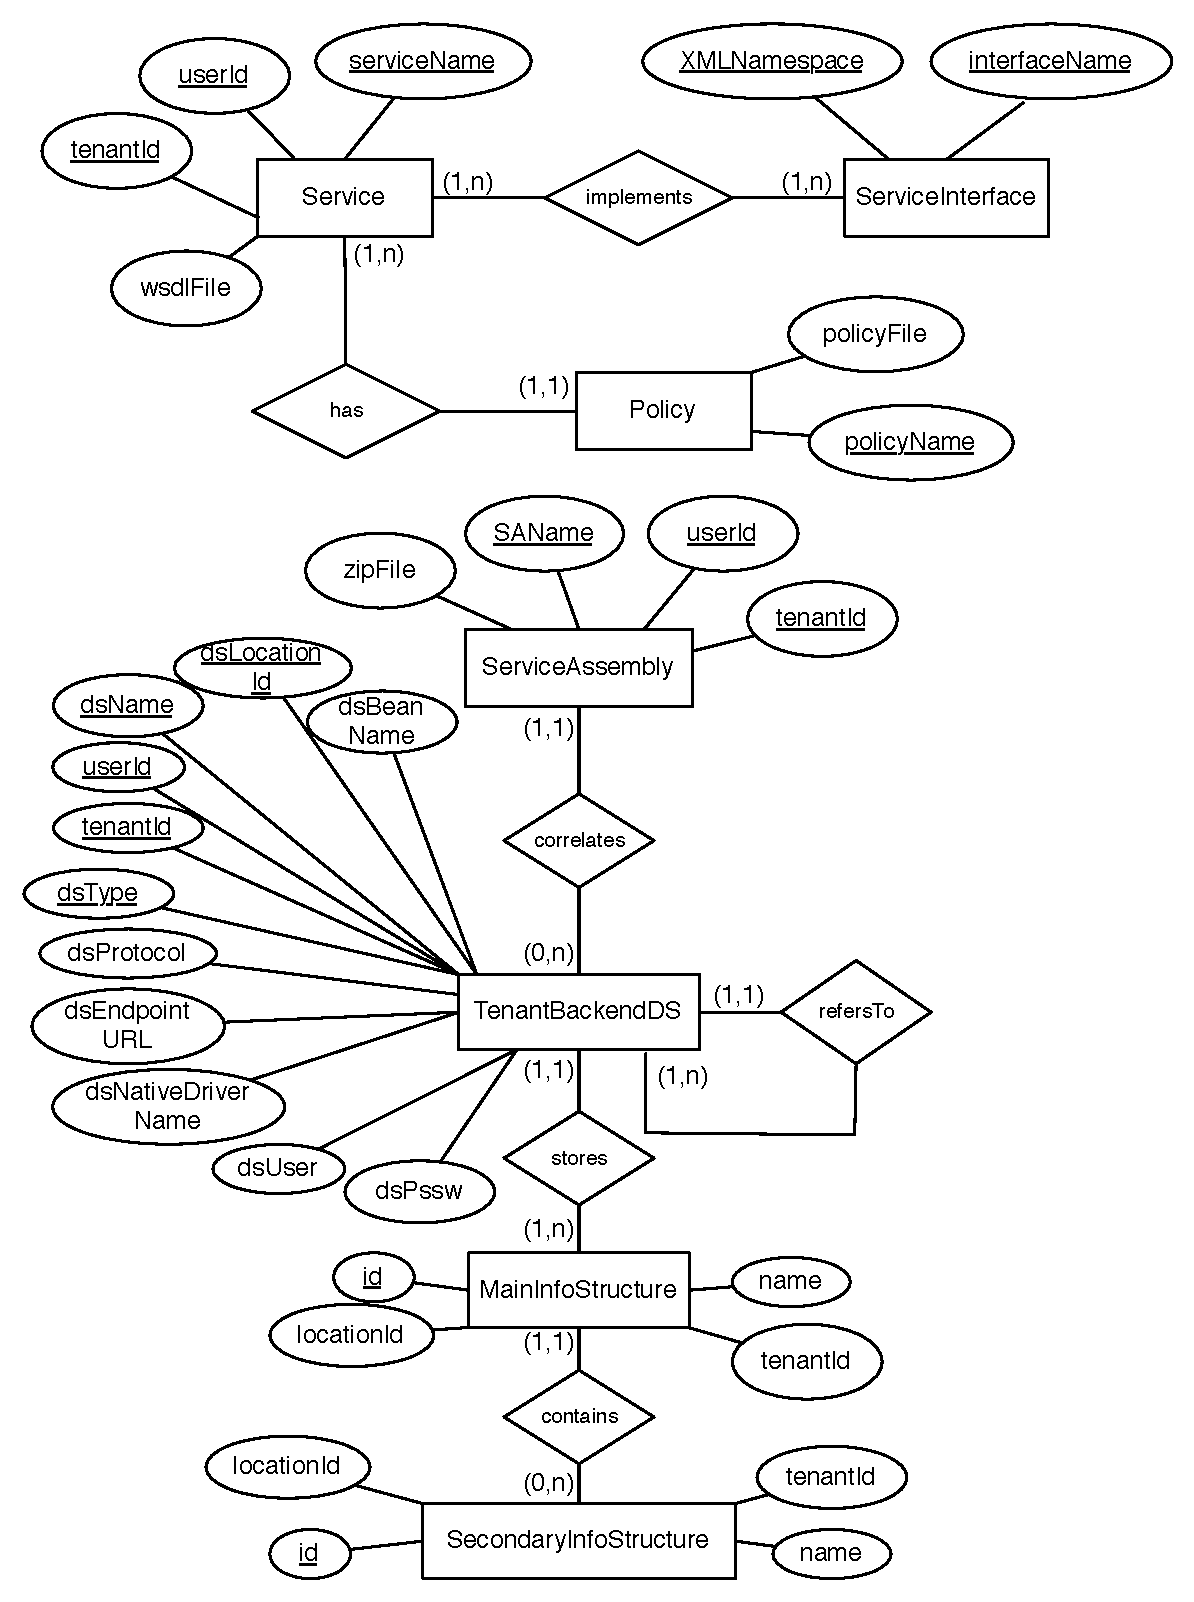
\includegraphics[clip, scale=0.7]{./gfx/dbModification/serviceRegistryV5_0_doc.pdf}
	\caption[Service Registry ER Diagram]{Extended service registry ER Diagram using (Min, Max) notation. Note: extended from outputs in \cite{Muhler2012} and \cite{Uralov2012}}
	\label{fig:serviceregistry}
\end{figure}

The service registry developed in Muhler's approach \cite{Muhler2012}, and extended in Uralov's work \cite{Uralov2012}, contains information related to the services, and policies which can be dynamically retrieved by the tenants. The services contains a WSDL file and implements an interface for its access. Furthermore, policies are attached to it in order to provide a dynamic discovery of services based on a set of rules. In this diploma thesis, we do not focus on service registering or service discovery, but on the endpoint configurations which are deployed by the tenants. These are stored in the service assembly entity, where the deployed \ac{SA}s are persisted with tenant context information. 

A \ac{SA} contains the \ac{SU}s where the endpoint configuration is described. Therefore, we consider the service assembly entity as the start point of our extension in the service registry schema. We use the data sources name to refer to the user's data sources, and categorize them as source or target data sources in the \term{dsLocationId} attribute. The  data source name in source data source registrations must equal to the database name the user includes in his request to CDASMix. Source data sources are the ones the tenant physically accesses in our system, while the target data sources are the ones that the tenant logically accesses, but the system physically accesses. Physical location of the target data sources are described in the \term{dsEndpointURL}, and define the database endpoint's host, port, and database name (an example is provided in Listing \ref{lst:testaddds}). A \ac{SA} contains the routing information configuration for routing operations between endpoints. Hence, one service assembly identifies the tenant's user source data sources. The source datasource can be connected to one or more target data sources, as shown in Figure \ref{fig:serviceregistry}. The self-referencing relation in the TenantBackendDS entity allows to reference one source data source with n target data sources.

As discussed in Chapter \ref{chap:relatedworks}, providing support for two different databases models, and for its different families (e.g. in \ac{NoSQL} databases) forces us to dissect their storage structures, and provide a generic and extensible model in order to store its meta-data. The \ac{SQL} data stores have two main storage structures: database and table. Inside the table we find a second storage structure, rows and columns. The \ac{NoSQL} databases are divided into different families, and for each family we find between the different vendors different namings which refer to the same storage structure. However, they all have in common the support of a main, and secondary storage structures. 

The data source entity stores the necessary information for providing access in the system, and for accessing the target databases in the target data sources. The configuration information is provided either by the tenant, or by the \term{Cloud Data Migration Application}, during and/or after the data migration process to the Cloud. We provide isolation in the registration of sensible information, e.g. access credentials, by indexing the table with the tenant and user \ac{UUID}. Whether transformation operations are required is detected by analyzing the value contained in the \term{dsType} attribute. The format of its value must comply the following standard: family-mainInfoStructure-secInfoStructure-version, e.g. sql-database-table-mysql5.1.2 for a MySQL database system, or nosqlKeyValue-bucket-object-1.0 for a bucket in Google Cloud Storage \cite{mysqlmanual}, \cite{googlecloudstorage}.  

The main information structure entity persists the data related to the database's main storage structure, e.g. table in MySQL databases, and table, bucket, or domain in \ac{NoSQL} databases. These storage structures are identified by its name in the backend data store. The locationid attribute in this entity categorizes one main information structure as source or target main information structure. A composite key formed by the name, locationid, and tenantid, is not possible in this entity. One tenant id may have the same name to identify two main information structure which are of a different database type, e.g. one \ac{SQL} table, and one \ac{NoSQL} bucket with the same name. Therefore, the entries in this entity are identified by a incremental id.   

The secondary information structure is used in our system only to persist meta-data for \ac{NoSQL} databases. The knowledge level in the system of tenant's migrated \ac{SQL} databases lowers to the table storage structure, and one database is uniquely associated with one tenant, user, and endpoint in the target database system, e.g in Amazon RDS one database is accessed by the database instance identifier, and the host name \cite{amazonrds}. However, different main storage structures can be accessed in \ac{NoSQL} databases through the same user's endpoint. Therefore, we need to persist one or more main storage structures per database system endpoint, and provide a second level, the secondary information structure, to register a tenant's \ac{NoSQL} database meta-data. For example, one tenant can create one or more buckets in the Google Cloud Storage system, and access them through the same endpoint \cite{googlecloudstorage}. Buckets store one or more objects, which are identified by their name. We must then associate a tenant's \ac{NoSQL} data store with one or more buckets, and these with one or more objects. A composite key formed by the name, tenantid, and locationid, is not possible, for the same reason discussed previously. One tenant id may have the same name to identify two secondary information structure which are of a different \ac{NoSQL} database type, e.g. one document, and one object with the same name. Therefore, the entries in this entity are identified by a incremental id.  As the relationships between secondary and main information structure, main information structure and data source, and between data sources (source and target) are a one to one relation, we avoid with the cascade option deleting   information which might be related with multiple entities, e.g. one target data source which is associated with two source data sources. 

The entities related to the upper entities, e.g. a second information structure related to a main information structure, and this to a data source, and to a service assembly, are set with the Java persistence property \term{Cascade}. The service assembly is the upper entity which defines the connection between one source, and multiple target data sources. The undeployment of a service assembly involves the deletion of the data sources which are related to the service assembly, and the main and secondary information structures. 

\FloatBarrier
\section{Normalized Message Format}
\label{sec:normalizedmessage}

In this diploma thesis we modify the \ac{NMF} design in \cite{gomez2012}, due to the different data types which are transferred in it. Gomez presents a \ac{NMF} where the data is transferred in its body in \ac{XML} format, which suites for the communication protocols his prototype supports (SOAP, JMS, and E-mail), and the text data type contained in the requests. Furthermore, the multi-tenant aware routing supported in his approach is static between endpoints (e.g. one incoming request is routed from one tenant's consumer endpoint to one tenant's provider endpoint). The complexity of the data types transferred in the system and the dynamic routing between backend Cloud data stores leads us to modify the meta-data transported in the \ac{NMF} properties section, and to send the data in the attachment section. We are also forced to design two different data structures for the \ac{NMF}: one for request messages, and another for response messages. The data and meta-data contained in the MySQL requests and responses messages require the utilization of different data structures to transmit them in the \ac{NMF} (see Listing \ref{lst:nmfcontent}). MySQL requests contain user, authentication, etc. meta-data, while the MySQL response contain meta-data which describes the data transferred. 

\begin{figure}[htb]
	\centering
		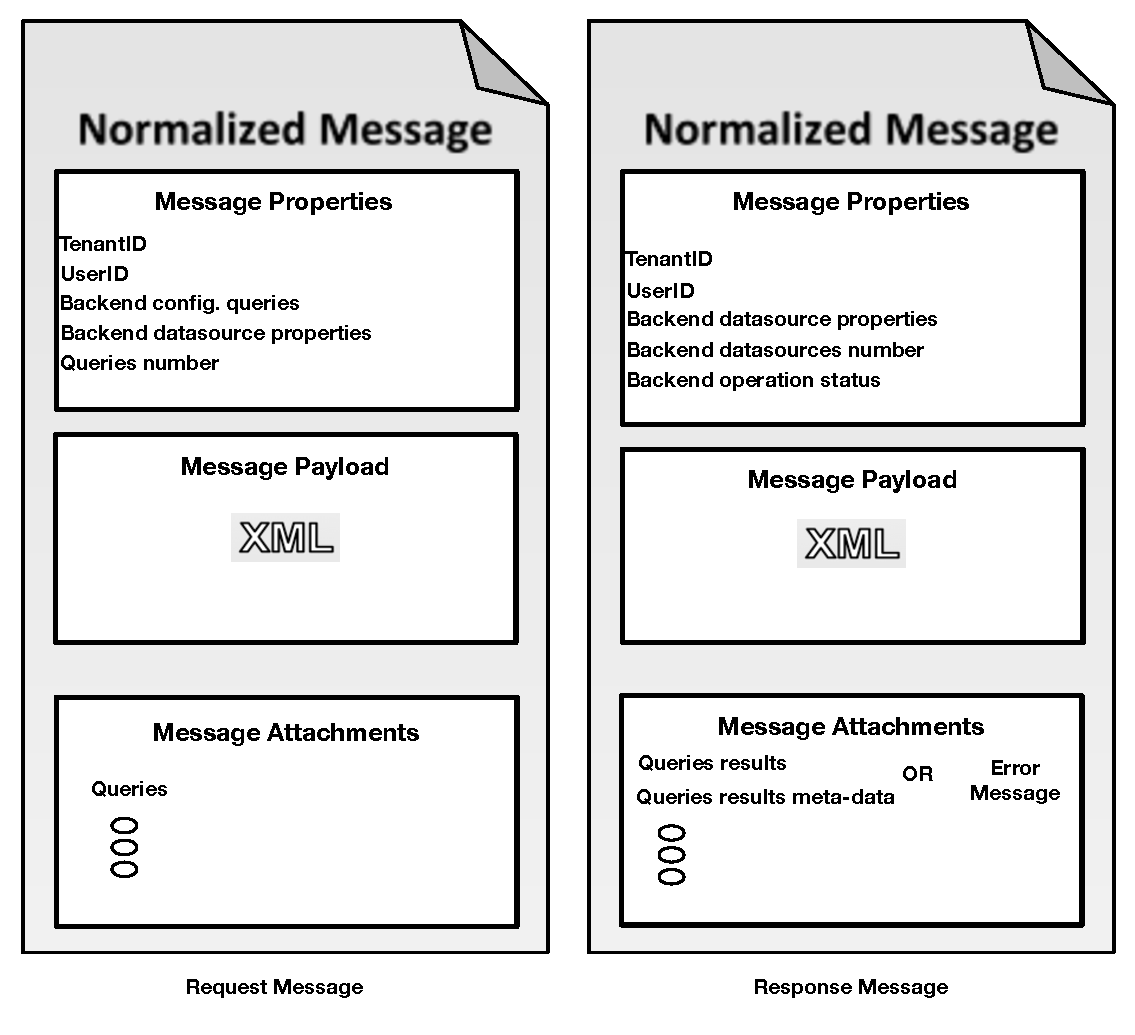
\includegraphics[clip, scale=0.7]{./gfx/normalizedMessage.pdf}
	\caption[Normalized Message Format Design]{Design of the Normalized Message Format used in the system.}
	\label{fig:nmf}
\end{figure}

Data access or modification requests to backend data stores through ServiceMix-mt are received in the vendor's communication protocol, e.g. MySQL communication protocol for MySQL database systems, or \ac{JSON} over \ac{HTTP} for \ac{NoSQL} databases, must be marshaled to the \ac{NMF} structure. The \ac{NMF} sections we use for incoming requests are the message properties, and the message attachment (see Figure \ref{fig:nmf}). In the message properties we attach tenant context information (tenant and user \ac{UUID}), and the request's meta-data, which is divided into:
	\begin{itemize}
		\item Backend configuration queries: server configuration queries sent prior to the request query, e.g. setting the predefined language, character encoding, etc. These must be executed in the backend database system, and are sent to the backend database system prior to the request query.
		\item Backend data source properties: in this property structure the set of backend data sources meta-data are stored, e.g. access credentials, main (and secondary) information structures names, data source type, etc.
		\item Queries number: the number of queries which are sent as attachment. The default value is one, but in multi-querying this value increases.
	\end{itemize}  

The \ac{NMF} body supports text data format. The data transferred to or retrieved from a backend Cloud data store is represented as different data types, e.g. string, integer, float, binary, etc., and must be transferred as binary data. Therefore, the queries contained in the user's requests are sent in the attachment section of the \ac{NMF}, which supports objects serialization. The queries are stored in a vector structure which can contain multiple queries. The \ac{NMF} request must be demarshaled to the appropriate database system's communication protocol before forwarding the user's request to the backend database system. 

Responses from the backend data stores are correlated with the user's request, marshaled, and sent back in the response \ac{NMF} (see Figure \ref{fig:nmf}). Data retrieved from a data store, e.g. in a data retrieval or update operation, contains both data and meta-data. Both informations are stored in vector structures in the attachment section of the response \ac{NMF}. In case of error, the error message is stored in the response \ac{NMF}, and forwarded back to the user. In the message properties section the tenant context information (tenant and user \ac{UUID}) is stored, and the response meta-data, which contains the following information:
	\begin{itemize}
		\item Backend data source properties: in this property structure the set of backend data sources meta-data are stored, e.g. main (and secondary) information structures names, data source type, etc.
		\item Backend data source number: the number of targeted data stores. 
		\item Backend operation status: the overall operation status. We consider operations over one or more target data stores as atomic. If one or more backend data stores returns an error, the operation status is set to error, and an error is forwarded back to the user. 
	\end{itemize}  

The message body may be used for sending structured data in \ac{XML} format. However, we do not send information in this \ac{NMF} section in this diploma thesis, due to the need to transfer the requests and response data as binary serializable objects (serializable vectors) in order to avoid errors in the data content if the data is transformed to string, and structured in XML format. 
\FloatBarrier
\section{SQL Support Architectural Overview}
\label{sec:designsql}

In this section we provide an overview of a preliminary, and final architectural approaches designed in this diploma thesis, in order to support a transparent data access to backend \ac{SQL} databases. We first expose the integration approaches we should consider, and the main problems found when implementing the first approach which led us to design a second architectural approach. 


\subsection{Integration}

%integration of osgi and jbi in terms of messaging
%integration of osgi and jbi in terms of containers and libraries
%explain why we have two approaches
%jbi components offered in servicmix are deployed as osgi bundles
% jbi components offered in servicemix-mt are deployed as jbi component, and internally wrapped into an osgi bundle
% may have to put a figure of the contents in both of the packages so that we can see. It is all about the meta inf library where the bundle manifest info is exposed
As described in Chapter \ref{chap:spec}, we build the new components in ServiceMix-mt following the \ac{OSGi} compliance. However, these must interact with components which follow the \ac{JBI} specification. The integration between components built for different containers in ServiceMix-mt must be done at two levels: messaging, and resources sharing. The ServiceMix-mt \ac{NMR} \ac{API} \ac{OSGi} bundle exposes a set of operations for sending messages through the \ac{NMR} to a specified target endpoint. Hereby we can perform message exchanges between endpoints configured on \ac{OSGi} bundles and endpoints configured on \ac{JBI} components, and provide communication support between components hosted in the two containers. 

\begin{figure}[htb]
	\centering
		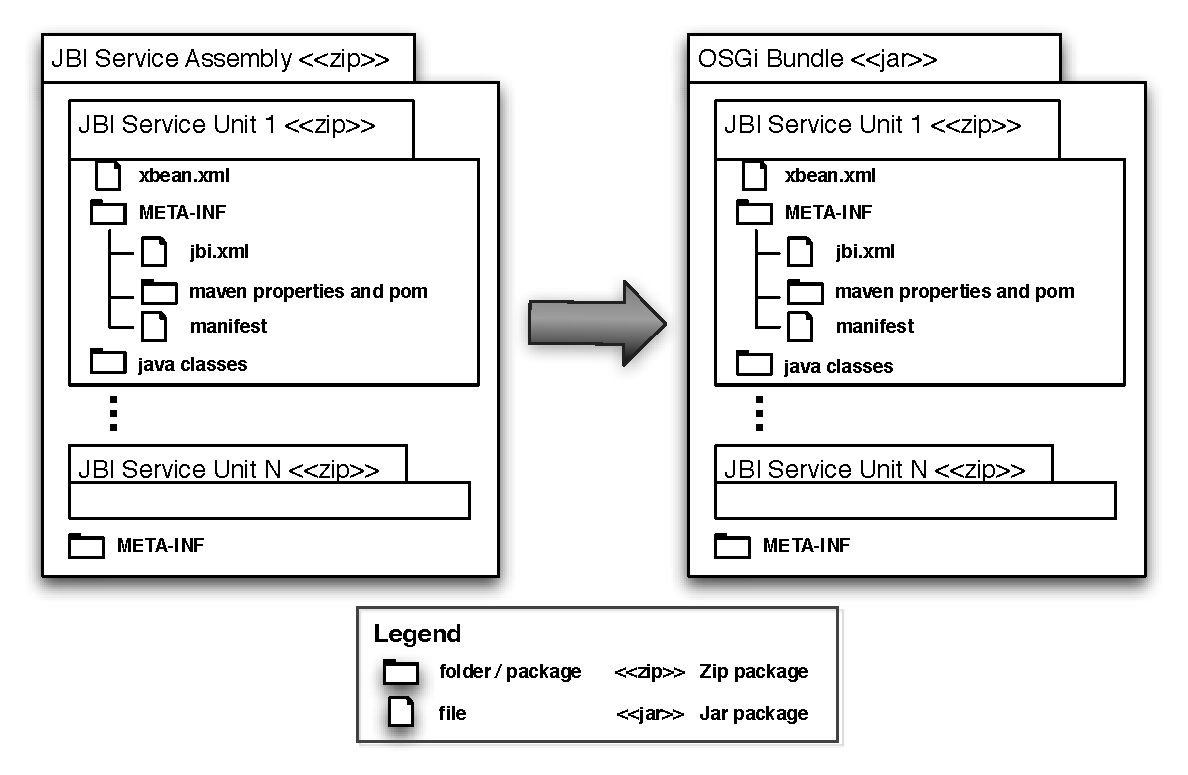
\includegraphics[clip, scale=0.5]{./gfx/osgibundlepackage.pdf}
	\caption[JBI to OSGi repackaging]{ServiceMix 4.x repackaging mechanism for deploying \ac{JBI} components in \ac{OSGi} container.}
	\label{fig:jbitoosgipackage}
\end{figure}

The resources sharing integration level refers to the deployment of \ac{JBI} components in the \ac{OSGi} container, and the utilization of packages exposed by \ac{OSGi} bundles in the \ac{OSGi} container in a loosely coupled manner. The former is part of the integration between containers provided in ServiceMix 4.x versions and described in Figure \ref{fig:jbitoosgipackage}. The deployment mechanism of a \ac{JBI} \ac{SA} into an \ac{OSGi} container is simple: repackaging of the \ac{SA} as a JAR. However, this cannot be consider a full integration in the \ac{OSGi} container. \ac{OSGi} bundles contain in their \term{META-INF} folder one fundamental file for the \ac{OSGi} kernel: the \term{manifest} file. This contains a description of the bundle, the packages it imports, and exports. Imported packages can be either statically stored in the bundle or imported from third party bundles, and exported packages are the ones which exposed to third party bundles. These can be imported with an internal class loading mechanisms developed in the \ac{OSGi} container. The repackaging of the \ac{SA} into a JAR, as it is shown in Figure \ref{fig:jbitoosgipackage}, contains the \term{META-INF} folder, and the \term{manifest} file. However, the latter only contains information about the author, date of creation, but it does not contain information related to the exported packages, and the needed packages to be imported. This \term{manifest} file describes the \ac{SA}, and not the \ac{SU}s. Java classes and package importing description are contained in the \ac{SU} package, and not in the \ac{SA} package. Therefore, the \ac{OSGi} container cannot register in its registry the packages it exports as a service, and cannot load the imported packages to the bundle context. This fact forces us to statically include in the \ac{SA}, and the \ac{SU} the packages which are referenced in each \ac{SU}, and leads to scalability constraints with the tenant-aware deployment process of the system.

ServiceMix 4.x versions are shipped with different \ac{JBI} \ac{BC}s packed as an \ac{OSGi} bundle. However, they are deployed as \ac{OSGi} bundles, and not as \ac{SA}s, in order to enable loose coupling and package sharing between components in the \ac{OSGi} container. ServiceMix-mt allows the deployment of the \ac{JBI} \ac{BC}s, but deployment of \ac{JBI} \ac{BC}s as OSGi bundles is not supported in the JBIMulti2 application. This lack of support forces us to design a second architectural approach, as described in the following sections.

\FloatBarrier

\subsection{Approach 1}

\ac{SQL} database systems provide access to their databases through an endpoint, which is represented as an URL. The native driver used in the data access layer of an application connects to the endpoint, authenticates, sends the query, and reads the response. Therefore, we must support in our system the same operational steps. As discussed in this diploma thesis, the communication protocol varies between different vendors. In this diploma thesis we provide support for incoming MySQL messages. Tenants must access our system through a single physical endpoint. This endpoint is provided by a MySQL proxy which is enriched with authentication, cashing, marshaling, and demarshaling operations. As shown in Figure \ref{fig:designsqlapp1}, the MySQL Proxy Bundle implements the MySQL server operations which are related with the client/server communication protocol. In Figure \ref{fig:designsqlapp1} we specify a server running on port 3306. However, this value can be configured before the deployment of the \ac{OSGi} component. This component is built as an \ac{OSGi} bundle and its packages are exported as services in the \ac{OSGi} container. It interacts with three different components in the system: the \ac{NMR} \ac{API}, the Cache, and the Service Registry. 

Cashing mechanisms are implemented in both the Registry-Cache, and the MySQL Proxy Bundle. The former provides an \ac{API} for creating cache instances, and for persisting and retrieving data. We create a separate cache instance for the \ac{SQL} support due to the need of a custom key creation mechanism which may not coexist in a shared cache between different bundles, as well as the needed isolation of sensible tenant configuration information from third party bundles. The system provides a set of operations which ease the creation of multi-tenant aware keys for persisting frontend authentication data, and queries results form the backend database systems. 

The \ac{NMR} \ac{API} is shipped in ServiceMix as an \ac{OSGi} bundle which exports its \ac{API} as an \ac{OSGi} service. The set of operations included in its \ac{API} allows \ac{OSGi} bundles to create, send, and receive message exchanges to \ac{JBI} endpoints (see Figure \ref{fig:designsqlapp1}).  Before creating the message exchange, the MySQL Proxy Bundle must build dynamically the target endpoint's URL by injecting the tenant context information, and service and endpoint name.

\begin{figure}[htb]
	\centering
		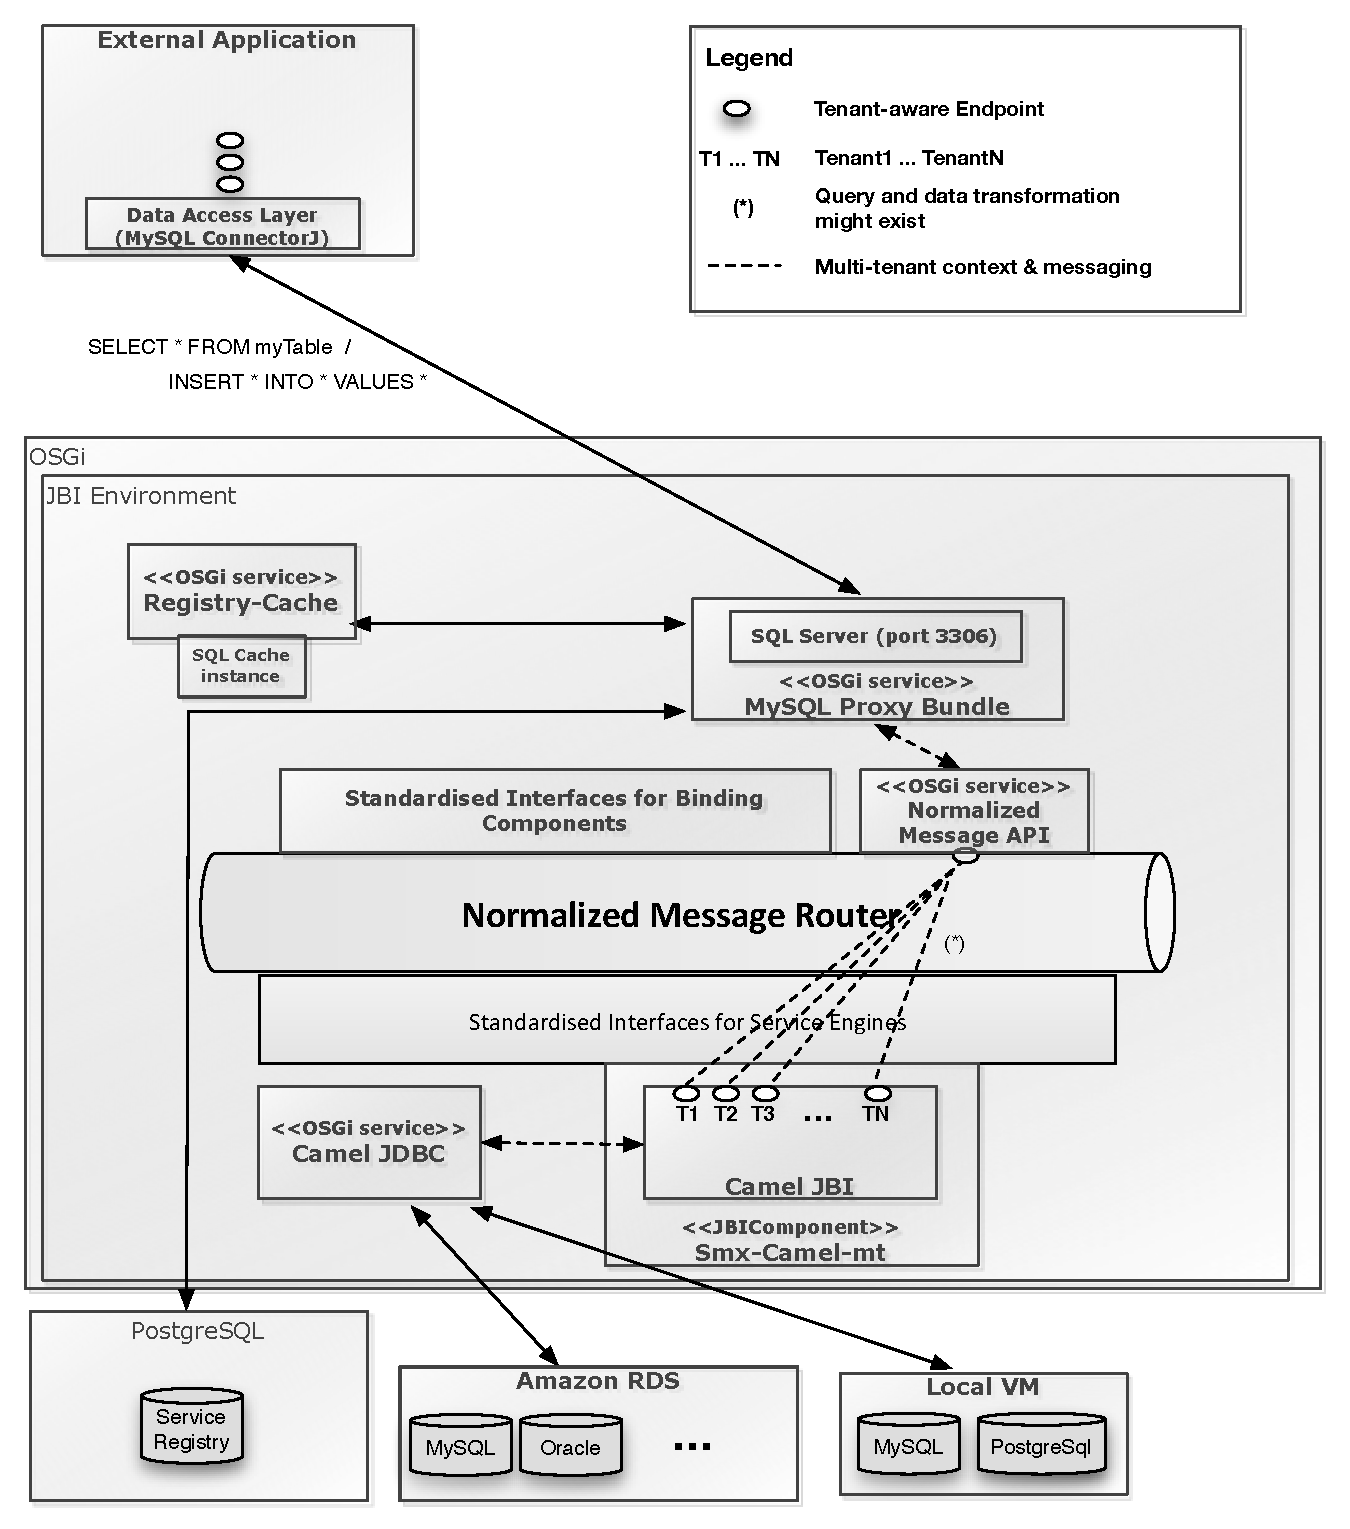
\includegraphics[clip, scale=0.6]{./gfx/sqlApproach/sqlApproachv2_doc.pdf}
	\caption[SQL Support Approach 1]{Architectural overview of the design approach one to support the MySQL communication protocol and routing to backend \ac{SQL} databases.}
	\label{fig:designsqlapp1}
\end{figure}

Apache Camel provides a set of components which integrate most of the communication technologies available in the market. Moreover, it provides an archetype for creating custom components we use in this diploma thesis. ServiceMix provides a Camel \ac{JBI} \ac{BC} which integrates the \ac{JBI} container with the camel router. Muhler extends this component in ServiceMix-mt and enriches it with multi-tenancy awareness. However, the supported multi-tenancy is at the level of tenants, and not at the level of tenant's users. We extend this component and provide user and tenant isolation between endpoints, by injecting the tenant and user UUID in the endpoint's URI (see Listing \ref{lst:endpointuri}). 

%%%%%%%%%%%%%%%%%%%%%%%%%%%%%
\lstinputlisting[float=htb,label={lst:endpointuri},caption={[Tenant-aware Endpoint Configuration]Extended Tenant-aware endpoint URI in extended Backus-Naur Form (EBNF) \cite{Muhler2012}.},style=ebnf]{./gfx/endpointconfiguration.txt}
%%%%%%%%%%%%%%%%%%%%%%%%%%%%%

With multi-tenancy at the tenant and user level, each user can deploy one \ac{JBI} tenant-aware endpoint in the ServiceMix-Camel-mt \ac{SE}. The routes deployed from each tenant-aware endpoint are performed under a different context, and an instance of the targeted component in the route is created. Therefore, with this approach we provide multi-tenancy at the messaging, endpoint, and routing and component context levels. 

Due to the lack of \ac{JDBC} support in ServiceMix for creating provider endpoints, we develop a custom camel component, and enrich it with \ac{JDBC} support for three database systems: MySQL, Oracle, and PostgreSQL. This component is extensible to more database systems when including its native driver, and is build as an \ac{OSGi} bundle and its packages are exported as an \ac{OSGi} service. Messages received from the \ac{NMR} are demarshaled to the backend database system communication protocol, and the response marshaled, correlated, and sent back to the MySQL Proxy Bundle. The demarshalers in this bundle provide the necessary support for transforming the \ac{NMF} response to a MySQL message.

As described in the previous section, ServiceMix-mt provides \ac{JBI} and \ac{OSGi} support and integration, but with some constraints. \ac{JBI} components cannot import packages from \ac{OSGi} bundles exporting its packages. The Servicemix-Camel-mt \ac{SE} provides integration with the camel router for a set of camel components. The camel manual specifies the need for adding statically the custom component packages in the \ac{JBI} \ac{SU} which contains the route definition. Therefore, this leads us to scalability problems in each of the \ac{SA} deployed by the tenants. The \ac{SA} size increases with the new supported database systems, and forces to redeploy all the \ac{SU}s containing the custom camel component when it is modified. This leads to management, storage capacity, and network capacity inconveniences. Hence, we provide a second, and final approach which is very similar to this one, but utilizing the ServiceMix-camel component deployed as \ac{OSGi} bundle. 

\FloatBarrier

\subsection{Approach 2}

In this second architectural design approach we address the scalability problems caused by the \ac{JBI} package dependencies in the \ac{SU}s described in the previous section. This approach is similar to the first one presented, and its main difference relies on the routing from the tenant-aware \ac{JBI} endpoints to the custom camel component \term{cdasmixjdbc} (see Figures \ref{fig:designsqlapp2} and \ref{fig:designsqlapp1}). The functionalities and operations in the MySQL proxy bundle do not differ with the previous approach.
 
\begin{figure}[htb]
	\centering
		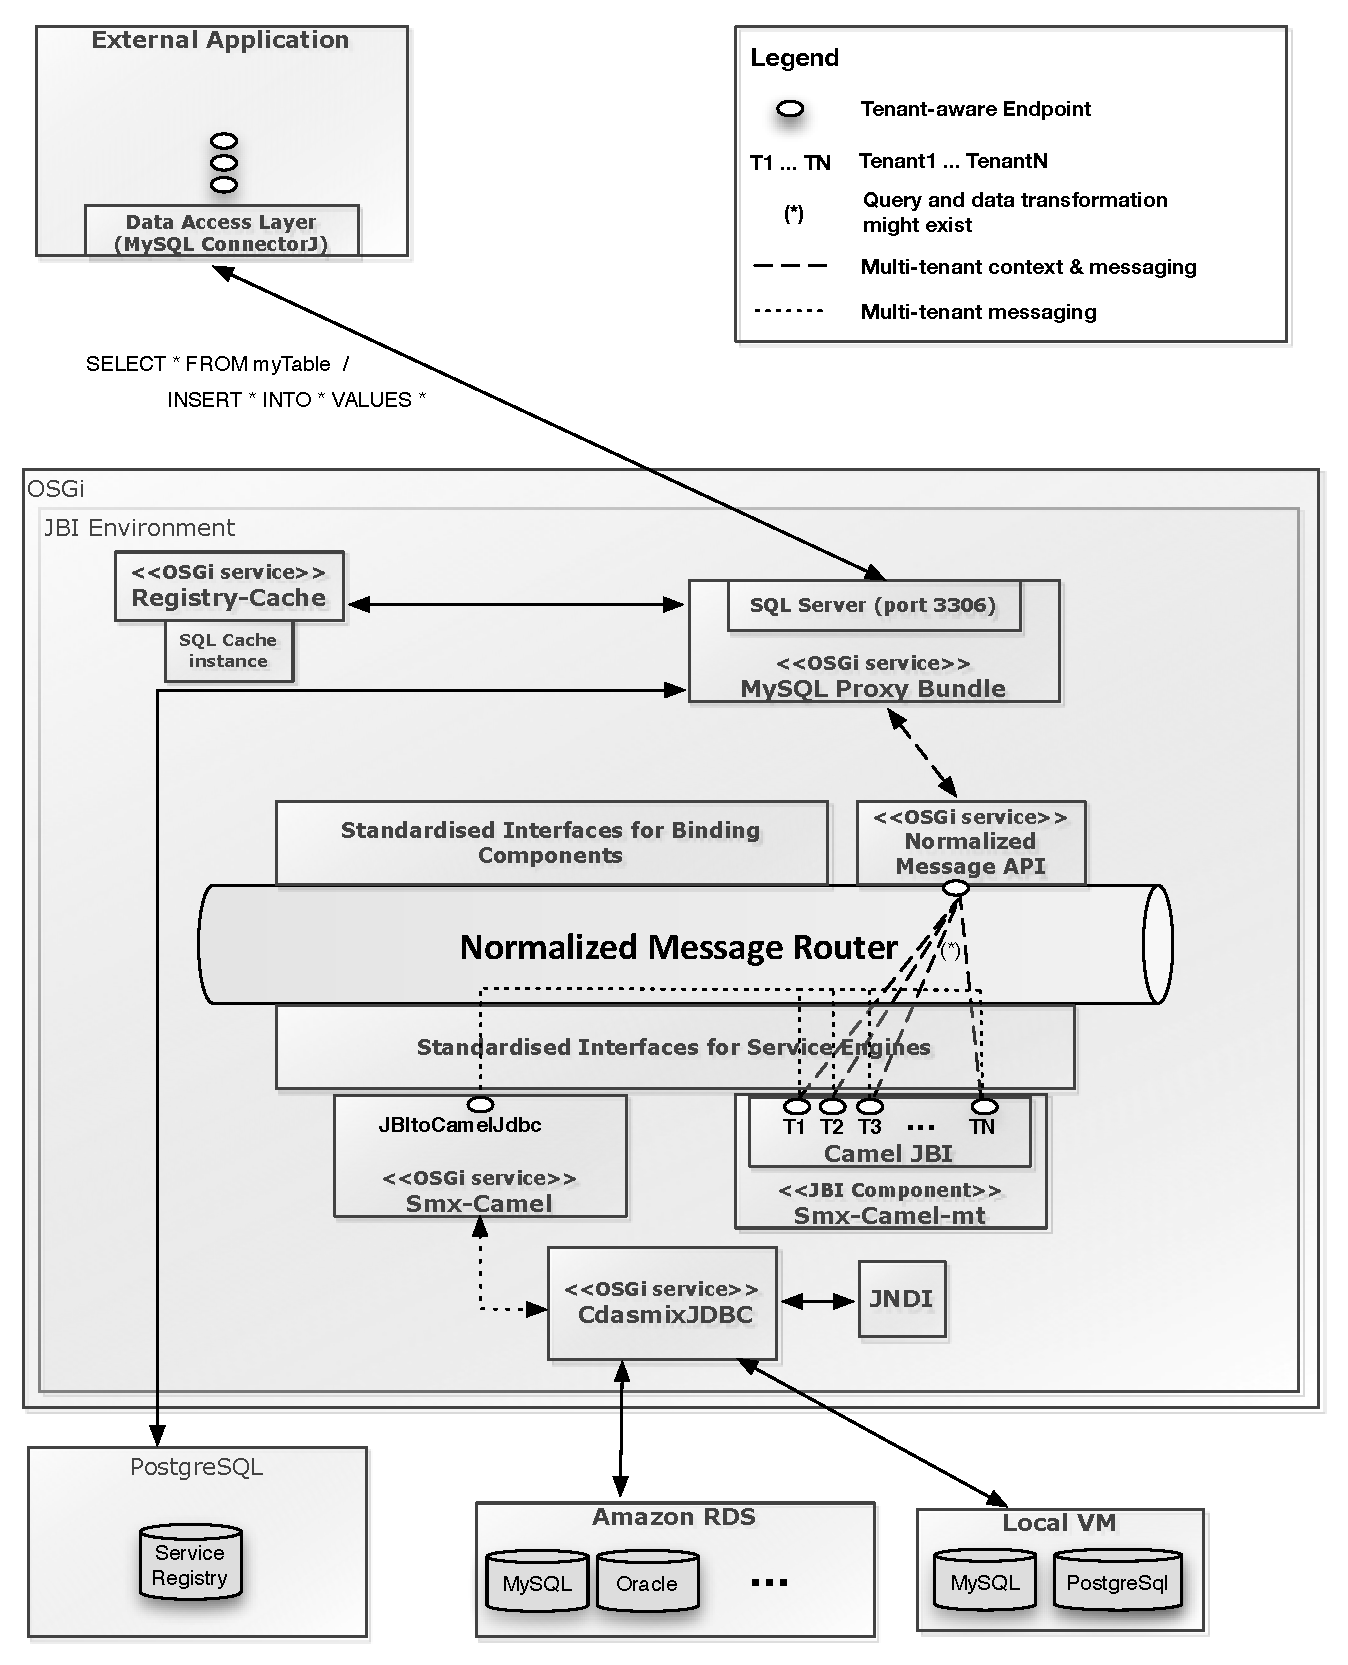
\includegraphics[clip, scale=0.6]{./gfx/sqlApproach/sqlApproachv3_doc.pdf}
	\caption[SQL Support Approach 2]{Architectural overview of the design approach two to support the MySQL communication protocol and routing to backend \ac{SQL} databases.}
	\label{fig:designsqlapp2}
\end{figure}

The message is routed from the MySQL proxy bundle to the tenant-aware \ac{JBI} endpoint deployed in ServiceMix-camel-mt. The multi-tenant message processor instance in ServiceMix-camel-mt routes the message to the \term{JBItoCamelJdbc} endpoint. 

As discussed before, the \ac{JBI} \ac{BC}s deployed in ServiceMix are \ac{OSGi} friendly. This means that the \ac{OSGi} contains a valid manifest file where the description of the bundle, import packages, and export packages are specified. \ac{SU}s deployed on this component are able to reference other \ac{OSGi} packages exposed as a service in the \ac{OSGi} service registry. We provide a single endpoint deployed in the ServiceMix-Camel component where the requests are sent to: the \term{JBItoCamelJdbc} endpoint. When the \term{JBItoCamelJdbc} endpoint is deployed on the ServiceMix-Camel \ac{OSGi} bundle, this searchs in the \ac{OSGi} container for the \term{CdasmixJDBC} component, and creates an instance of the component. Messages routed to the \term{JBItoCamelJdbc} endpoint are then forwarded to the \term{CdasmixJDBC} component, which selects the appropriate \ac{JDBC} native driver, creates a connection, demarshals the request, and forwards the request to the backend Cloud data store server. The connection is established after creating an instance of a \term{DataSource}, which is saved in the \ac{JNDI} registry for future connections, in order to avoid the creation of more than one \term{DataSource} instance per user per backend Cloud data store.

Responses retrieved from the backend Cloud data store are correlated with the initial request and routed back to the MySQL proxy bundle, which demarshals the retrieved data and sends it as a binary \ac{TCP} stream.

In this approach a new instance of the \term{cdasmixjdbc} is not created per tenant endpoint, but is shared between the tenants. Therefore, we cannot ensure an independent component context at the provider endpoint. However, messages contain the tenant information, and the \term{cdasmixjdbc} component interacts with the backend database system establishing separate \ac{JDBC} connections per request. Full multi-tenancy, at the levels of component creation, and endpoint level is not ensured, but it is ensured at the messaging, and context levels. Although full multi-tenancy is not supported, we avoid the deployment of \ac{SU}s which contain the \term{CdasmixJDBC} component in it, and whose size increase may lead to scalability problems in the system. Furthermore, we prevent the deployment of the same component n times, for the n multi-tenant aware endpoints, and prevent future management problems when modifying or upgrading the \term{CdasmixJDBC} component. 

\FloatBarrier



\section{NoSQL Databases}
\label{sec:fundamentalsnosqldb}  

\ac{RDBMS}s ensure data persistency over time and provide a wide set of features. However, the functionalities supported require a complexity, which is sometimes not needed for some applications, and harms important requirements in Web applications or in \ac{SOA} based applications, e.g. throughput. \ac{NoSQL} data stores aim to improve the efficiency of large amount of data storage while reducing its management cost \cite{nosqlcomputerworld}. NoSQL databases are designed to support horizontal scalability without relying on the highly available hardware \cite{strauchnosql}. In a Cloud storage environment where the user sees the available computing and storage resources as unlimited, a \ac{NoSQL} support in a Cloud storage environment might be adequate.

\ac{NoSQL} \ac{DBS} operate as a schema-less storage system, allowing the user to access, modify or freely insert his data without having to make first changes in the data structure \cite{nosql2012}. Cloud providers provide the users with an \ac{API} for accessing, modifying, and inserting data into his isolated container. For example, a user's Amazon Dynamo DB table and item can be accessed by its RESTful \ac{API}, or by installing at the user's side application the Amazon Web Services SDK \cite{amazondynamodb}. Furthermore, it provides the users through its Web-based management console the available management operations. 

Due to the growth of the \ac{NoSQL} support along different Cloud vendors, in this diploma thesis we provide a multi-tenant and transparent communication support for \ac{NoSQL} backend data stores in different Cloud providers. In the following sections we introduce the categorization of the different \ac{NoSQL} databases we aim to support in this diploma thesis, mentioning and giving examples of Cloud data stores available nowadays in the market.

\subsection{Key-value Databases}

In a key-value datastore elements are uniquely identified by an id, which the data store does not take into account its type, and are simply stored as a \ac{BLOB} . A user can get the value for the key, put a value for the key, or delete a key from the data store \cite{nosql2012}. Its storage model can be compared to a map/dictionary \cite{strauchnosql}. Products offering this data storage model in a Cloud infrastructure are Amazon DynamoDB \cite{amazondynamodb}, Google Cloud Storage \cite{googlecloudstorage}, Amazon SimpleDB  \cite{amazonsimpledb} , Amazon S3 \cite{amazons3}, etc. In this diploma thesis we mainly focus on the following key-value data stores: DynamoDB, and Google Cloud Storage.

Amazon DynamoDB's data model includes the following concepts: tables, items, and attributes \cite{amazondynamodb}. The attributes are a key-value, where the value is binary data. Attributes are stored in items, and these are stored in tables. Items stored in a table can be retrieved by referencing its unique id. The number of attributes is not limited by Amazon, but each item must have a maximum size of 64 KB. Accessing stored data in this data store can be mainly done in two ways: using the functionalities provided by the AWS SDK, or using the Cloud storage RESTful \ac{API}. 

Google Cloud Storage's data model includes the following concepts: buckets and objects \cite{googlecloudstorage}. Buckets contain on or more objects. The objects are identified within a bucket with its unique id. Users can perform I/O operations on both buckets and objects. For this purpose, Google Cloud storage provides RESTful \ac{API}.

In this diploma thesis we use an \ac{ESB} for accessing transparently tenant's databases migrated to the Cloud. Servicemix-mt provides multi-tenant \ac{HTTP} support \cite{gomez2012}. Therefore, we reuse and extend the multi-tenant \ac{HTTP} \ac{BC} in order to provide dynamic routing between the different data stores.

\subsection{Document Databases}

Document databases can be considered as a next step in improving the key-value storage model. In this storage model, documents are stored in the value part of the key-value store, making the value content examinable \cite{nosql2012}. Documents with different schemas are supported in the same collection, and can be referenced by the collection's key or by the document's attributes. One of the main difference in the attributes specification regarding \ac{RDBMS} is that in document stores document's attributes cannot be null. When there is an attribute without value, the attribute does not exist in the document's schema. Products implementing this data storage model are Apache CouchDB, MongoDB, etc. \cite{couchdb} \cite{mongodb}.

Mongo DB defines two storage structures: collections and documents \cite{mongodb}. A specific database contains one or more collections identified by its unique id. A specific collection stores one or more documents. Collections and documents stored in a database can be accessed, inserted and modified using the RESTful \ac{API} supported by the database system.

Apache CouchDB defines two storage structures: databases and documents. Data stored in CouchDB are \ac{JSON} documents. The main difference between this two described databases is that MongoDB implements a two step access to the documents: database, collection, and document. Apache CouchDB provides a RESTful \ac{API} for I/O operations.

This databases are not offered by Cloud providers like Amazon or Google, but as a software which can be deployed in user instances, e.g. Amazon EC2 AMI \cite{amazonec2}. 

\subsection{Column-family Stores}

One of the most known Column-family data stores is Cassandra. Column-family data stores store data in column families (groups of related columns which are often accessed together) as rows that have many columns associated with a row key \cite{nosql2012}. This approach allows to store and process data by column instead of by row, providing a higher performance when accessing large amount of data, e.g. allowing the application to access common accessed information in less time.

Cassandra has as its smallest unit of storage the column, which consists of a timestamp and a name-value pair where the name acts as a key \cite{nosql2012}. As in the relational model, a set of columns form up a row, which is identified by a key. A column family is a collection of similar rows. The main difference with the relational model is that each of the rows must not have the same columns, allowing the designer and the application consuming large amounts of data to customize the columns in each row, and the rows in each column family.

Cassandra is not shipped with a RESTful API for I/O operations. However, there are several open-source services layers for Cassandra, e.g. Virgil \cite{virgil}.

\FloatBarrier


\FloatBarrier